
\section{Experimental results}
\label{sec:experimental-results}
% <<<<<<< HEAD
% \begin{table}[t]
%   \centering
%   \twocolumn[

%   \begin{@twocolumnfalse}
%     \caption{Benchmark programs using \texttt{delay} constructs} \label{table:benchmark}
%     \scalebox{0.85}{
%       \begin{tabular}{|c| c | c | c | c | c | c | c |}
% 	\cline{4-8}
% 	\multicolumn{3}{c|}{}											& HRTCS 		& Motor 		  & Robot 			  & AECS/CD1  		   & AECS/CD2\\ \hline
% 	\multirow{12}{*}{JOP} 		& \multicolumn{2}{|c|}{BCRT} 		&0.0334 ms 		& 0.0361 ms		  & 0.0325 ms		  & 0.1683 ms		   & 0.1881 ms\\ \cline{2-8}   
%         & \multicolumn{2}{|c|}{WCRT} 		&0.1120 ms 		& 0.1116 ms		  & 0.0601 ms		  & 0.7147 ms		   & 1.0115 ms\\ \cline{2-8} 
%         & \multirow{2}{*}{Delay 1}	 & M..N &50.3-200.3 ms 	& 2.4-7.4772 ms	  & 1230-2274.0263 ms & 10000-42473.2197 ms& 10000-53772.0045 ms \\ \cline{3-8} 
%         &			   & d			 		&1506-1787  	& 67 			  & 37861			  & 59427		       &53160\\ \cline{2-8}
%         & \multirow{2}{*}{Delay 2}	 & M..N & 	N/A 		& 1.667-5.2452 ms & N/A				  & N/A 			   &10000-53772.0045 ms\\ \cline{3-8} 
%         &			   & d			 		& 	N/A	 		& 47			  & N/A				  & N/A       		   &53160\\ \cline{2-8}
%         & \multirow{2}{*}{Delay 3}	 & M..N & 	N/A	 		& 0.05-0.2232 ms  & N/A				  & N/A       		   &N/A\\ \cline{3-8} 
%         &			   & d			 		& 	N/A	 		& 2		      	  &	N/A				  & N/A       		   &N/A\\ \cline{2-8}
%         & \multirow{2}{*}{Delay 4}	 & M..N & 	N/A	 		& 0.3-1.0044 ms   & N/A				  &	N/A       		   &N/A\\ \cline{3-8} 
%         &			   & d				 	& 	N/A	 		& 9				  & N/A				  &	N/A      		   &N/A\\ \cline{2-8}
%         & \multirow{2}{*}{Delay 5}	 & M..N & 	N/A	 		& 0.733-2.3436 ms & N/A				  &	N/A      		   &N/A\\ \cline{3-8} 
%         &			   & d			 		& 	N/A	 		& 21 			  &	N/A				  & N/A      		   &N/A\\ \hline
% 	\multirow{12}{*}{TP-JOP} 	& \multicolumn{2}{|c|}{BCRT} 		&0.0028 ms 		& 0.0060 ms		  & 0.0011 ms		  & 0.0532 ms		   & 0.0292 ms\\ \cline{2-8}   
%         & \multicolumn{2}{|c|}{WCRT} 		&0.0329 ms 		& 0.0393 ms		  & 0.0361 ms		  & 0.5072 ms		   & 0.8388 ms\\ \cline{2-8} 
%         & \multirow{2}{*}{Delay 1}	 & M..N &50.3-600.3 ms 	& 2.4-15.6265 ms  & 1230-42317.8276 ms& 10000-95358.8578 ms& 10000-287757.9834 ms \\ \cline{3-8} 
%         &			   & d			 		&18209-18232 	& 398 			  & 1171429			  & 188015		       &343054\\ \cline{2-8}
%         & \multirow{2}{*}{Delay 2}	 & M..N & 	N/A 		& 1.667-10.8757 ms& N/A				  & N/A 			   &10000-287757.9834 ms\\ \cline{3-8} 
%         &			   & d			 		& 	N/A	 		& 277			  & N/A				  & N/A       		   &343054\\ \cline{2-8}
%         & \multirow{2}{*}{Delay 3}	 & M..N & 	N/A	 		& 0.05-0.3534 ms  & N/A				  & N/A       		   &N/A\\ \cline{3-8} 
%         &			   & d			 		& 	N/A	 		& 9		      	  &	N/A				  & N/A       		   &N/A\\ \cline{2-8}
%         & \multirow{2}{*}{Delay 4}	 & M..N & 	N/A	 		& 0.3-1.9631 ms   & N/A				  &	N/A       		   &N/A\\ \cline{3-8} 
%         &			   & d				 	& 	N/A	 		& 50			  & N/A				  &	N/A      		   &N/A\\ \cline{2-8}
%         & \multirow{2}{*}{Delay 5}	 & M..N & 	N/A	 		& 0.733-4.79 ms   & N/A				  &	N/A      		   &N/A\\ \cline{3-8} 
%         &			   & d			 		& 	N/A	 		& 122 			  &	N/A				  & N/A      		   &N/A\\ \cline{2-8}
% 	\hline
%       \end{tabular}
%     }
%   \end{@twocolumnfalse}
%   ]

% \end{table}
% In this section, we present a set of SystemJ benchmark programs in which
% real-time requirements should be met.  We have carried out a set of
% experiments to obtain BCRT and WCRT of the benchmark programs on two
% execution platforms called Java Optimized Processor(JOP)
% \cite{jop:jnl:jsa2007} and TP-JOP \cite{6119095}. JOP is a hardware
% implementation of the JVM which enables real-time execution of Java
% programs by translating Java bytecodes into a sequence of JOP's native
% instructions called \emph{microcode} which is time-predictable. As
% SystemJ's default compilation target is Java source code, JOP is an
% excellent platform which enables us to analyze timing properties of
% SystemJ program. On the other hand, there is also an option where
% compiled code could be more tightly coupled to specific platforms such
% as TP-JOP, which execute SystemJ's kernel statements more
% efficiently. By utilizing our internal tools in conjunction with
% Worst-Case-Execution-Time (WCET) analyzer \cite{jop:jnl:jsa2007}
% provided by JOP tools, we were able to estimate BCRT and WCRT of our
% benchmark programs: (full-name?) HRTCS, Stepper motor controller (Motor)
% \cite{}, Robot and Access Environment Control System (AECS) \cite{}.

% % HRTCS, as already illustrated in Section \ref{sec:intr-motiv}, tests
% % for an ability of one's responsiveness by generating green lights
% % between the real-time range \emph{M - N}. For AECS \ref{} we have
% % replaced the external timer with our delay constructs. Stepper motor
% % controller is originally introduced in \cite{Bourke2009a} which
% % converted into SystemJ.

% As one can see in Table \ref{table:benchmark}, BCRT and WCRT of overall
% programs are smaller when they run on TP-JOP. For example, WCRT and BCRT
% of HRTCS are \(\times\)11.9 and \(\times\)3.4 smaller, respectively, for
% TP-JOP (0.0028, 0.0329 ms) compared to JOP (0.0334, 0.1120 ms). On the
% other hand, required logical delays \emph{d} are generally bigger on
% TP-JOP e.g. \(\times\)4.5 - \(\times\)5.9 and \(\times\)30.9 in Motor
% and Robot respectively. It is expected as their BCRT and WCRT
% differences are bigger on TP-JOP.  This also led to greater increase in
% minimum upper real-time bounds \emph{N} for TP-JOP in every example.  In
% AECS, there are two clock-domains using delay constructs that each has
% their own BCRT and WCRT. Again, individual BCRT and WCRT is smaller
% whereas \emph{d} is bigger on TP-JOP. One important property to note
% here, is that BCRT and WCRT of any clock-domains are invariant of
% \emph{d} as explained in Section \ref{sec:intr-real-time}. It is our
% fundamental assumption to find \emph{d} in our benchmark programs.
% =======

\begin{table}[t]
\twocolumn[
\centering
\begin{@twocolumnfalse}
\caption{Benchmark programs using \texttt{delay} constructs} \label{fig:comparison}
\resizebox{18cm}{2.4cm}{
\begin{tabular}{| c | c | c | c | c | c | c |}
	\cline{3-7}
	\multicolumn{2}{c|}{}											& HRTCS 		& Motor 		  & Robot 			  & AECS/CD1  		   & AECS/CD2\\ \hline
								 \multicolumn{2}{|c|}{BCRT} 		&0.0334 ms 		& 0.0361 ms		  & 0.0325 ms		  & 0.1683 ms		   & 0.1881 ms\\ \cline{1-7}
								 \multicolumn{2}{|c|}{WCRT} 		&0.1120 ms 		& 0.1116 ms		  & 0.0601 ms		  & 0.7147 ms		   & 1.0115 ms\\ \cline{1-7}
								 \multirow{2}{*}{Delay 1}	 & M..N &50.3-200.3 ms 	& 2.4-7.4772 ms	  & 1230-2274.0263 ms & 10000-42473.2197 ms& 10000-53772.0045 ms \\ \cline{2-7}
											   & d			 		&1506-1787  	& 67 			  & 37861			  & 59427		       &53160\\ \cline{1-7}
								 \multirow{2}{*}{Delay 2}	 & M..N & 	N/A 		& 1.667-5.2452 ms & N/A				  & N/A 			   &10000-53772.0045 ms\\ \cline{2-7}
											   & d			 		& 	N/A	 		& 47			  & N/A				  & N/A       		   &53160\\ \cline{1-7}
								 \multirow{2}{*}{Delay 3}	 & M..N & 	N/A	 		& 0.05-0.2232 ms  & N/A				  & N/A       		   &N/A\\ \cline{2-7}
											   & d			 		& 	N/A	 		& 2		      	  &	N/A				  & N/A       		   &N/A\\ \cline{1-7}
								 \multirow{2}{*}{Delay 4}	 & M..N & 	N/A	 		& 0.3-1.0044 ms   & N/A				  &	N/A       		   &N/A\\ \cline{2-7}
											   & d				 	& 	N/A	 		& 9				  & N/A				  &	N/A      		   &N/A\\ \cline{1-7}
								 \multirow{2}{*}{Delay 5}	 & M..N & 	N/A	 		& 0.733-2.3436 ms & N/A				  &	N/A      		   &N/A\\ \cline{2-7}
											   & d			 		& 	N/A	 		& 21 			  &	N/A				  & N/A      		   &N/A\\ \hline
% 	\multirow{12}{*}{TP-JOP} 	& \multicolumn{2}{|c|}{BCRT} 		&0.0028 ms 		& 0.0060 ms		  & 0.0011 ms		  & 0.0532 ms		   & 0.0292 ms\\ \cline{2-8}
% 								& \multicolumn{2}{|c|}{WCRT} 		&0.0329 ms 		& 0.0393 ms		  & 0.0361 ms		  & 0.5072 ms		   & 0.8388 ms\\ \cline{2-8}
% 								& \multirow{2}{*}{Delay 1}	 & M..N &50.3-600.3 ms 	& 2.4-15.6265 ms  & 1230-42317.8276 ms& 10000-95358.8578 ms& 10000-287757.9834 ms \\ \cline{3-8}
% 								&			   & d			 		&18209-18232 	& 398 			  & 1171429			  & 188015		       &343054\\ \cline{2-8}
% 								& \multirow{2}{*}{Delay 2}	 & M..N & 	N/A 		& 1.667-10.8757 ms& N/A				  & N/A 			   &10000-287757.9834 ms\\ \cline{3-8}
% 								&			   & d			 		& 	N/A	 		& 277			  & N/A				  & N/A       		   &343054\\ \cline{2-8}
% 								& \multirow{2}{*}{Delay 3}	 & M..N & 	N/A	 		& 0.05-0.3534 ms  & N/A				  & N/A       		   &N/A\\ \cline{3-8}
% 								&			   & d			 		& 	N/A	 		& 9		      	  &	N/A				  & N/A       		   &N/A\\ \cline{2-8}
% 								& \multirow{2}{*}{Delay 4}	 & M..N & 	N/A	 		& 0.3-1.9631 ms   & N/A				  &	N/A       		   &N/A\\ \cline{3-8}
% 								&			   & d				 	& 	N/A	 		& 50			  & N/A				  &	N/A      		   &N/A\\ \cline{2-8}
% 								& \multirow{2}{*}{Delay 5}	 & M..N & 	N/A	 		& 0.733-4.79 ms   & N/A				  &	N/A      		   &N/A\\ \cline{3-8}
% 								&			   & d			 		& 	N/A	 		& 122 			  &	N/A				  & N/A      		   &N/A\\ \cline{2-8}
% 	\hline
\end{tabular}
}
\end{@twocolumnfalse}
]
\end{table}

% \begin{figure}
% \centering
% 	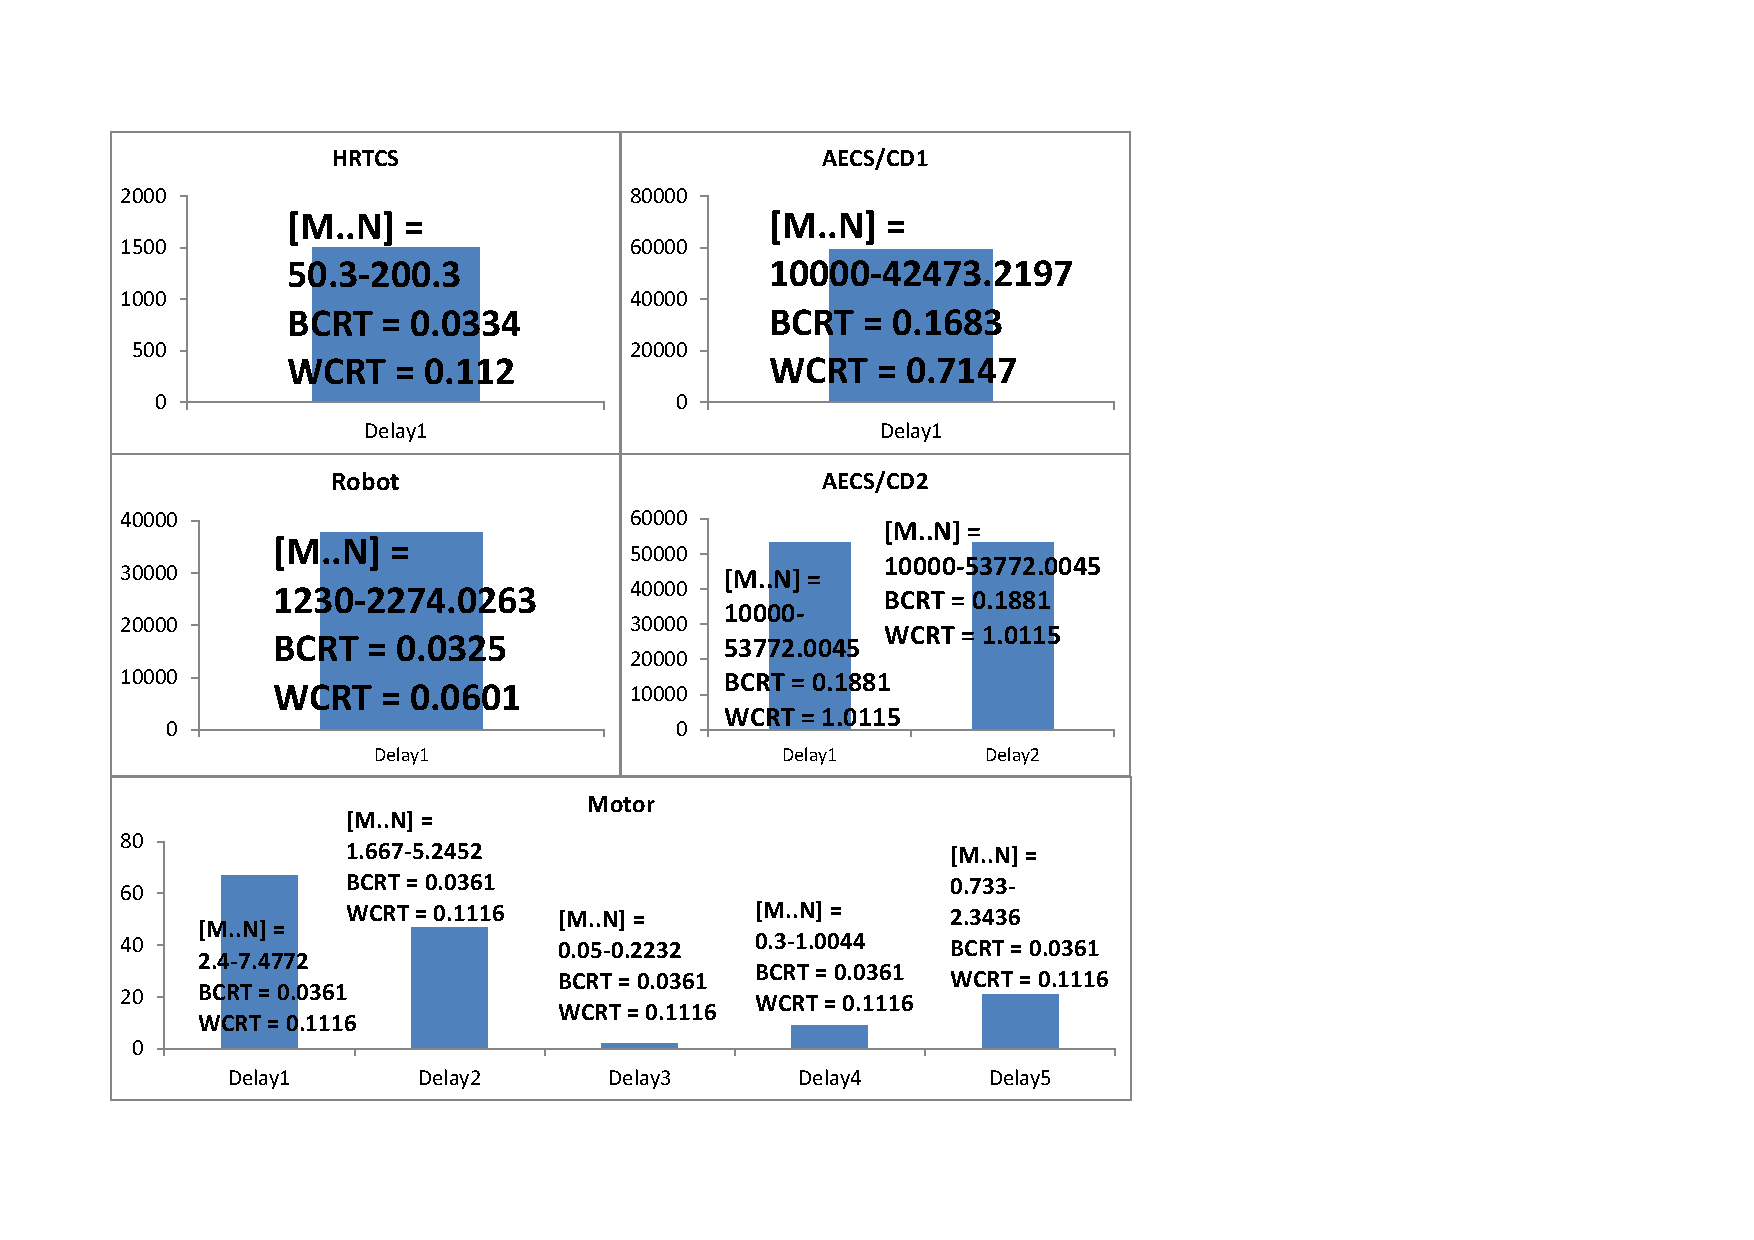
\includegraphics[trim=2cm 2cm 2cm 2cm,scale=0.5]{table2}
%         \caption{Evaluation of logical delays \emph{d} for on various
%           benchmark programs}\label{fig:comparison}
% \end{figure}


We have carried out a number of experiments on a set of applications
with real-time constraints. The benchmark set is shown in
Table~\ref{fig:comparison}. HRCTS is the human response system described
in Figure~\ref{fig:1}. AECS (Access and Environmental Control System) is
an application that controls an intelligent room environment described
in~\cite{aecs_ispa}. The system interacts with two external timers
through input/output signals in order to measure how long the entrance
door to the room is being opened and time the illegal presence (e.g.
intruder) that is being detected. The program has been modified such
that the delay constructs are used instead of external timers as shown
in~\ref{delaycode}.


\begin{figure}[h!]
	\begin{SubFloat}{\label{delaycode:a}sss}
		\centering
		\begin{minipage}[b]{0.3\linewidth}
			\footnotesize
\begin{verbatim}
emit TimerTriggered;
trap(T){
  abort(DoorOpened){
    await(TimeOut);
    exit(T); 
  }
}
\end{verbatim}
		\end{minipage}
	\end{SubFloat}
\hspace{1cm}%
	\begin{SubFloat}{\label{delaycode:b}sss}
		\centering
		\begin{minipage}[b]{0.3\linewidth}
			\footnotesize
\begin{verbatim}
// No emit statement
trap(T){
  abort(DoorOpened){
    delay(2.4 .. 7.4772 ms);
    exit(T);  
  }
}
\end{verbatim}
		\end{minipage}
	\end{SubFloat}
\caption{www}
\label{delaycode}
\end{figure}


Motor is a stepper motor controller from~\cite{Bourke2009a}. Robot is an
industrial automation application that consists of two manufacturing
belts and a robotic arm that splits goods according to their volumes.
HRCTS consists of 2 CDs, but only one with real-time delays. AECS also
has 2 CDs; CD1 consist of a single delay statement, while CD2 has 2
delay statements. Robot and Motor both are synchronous programs with 1
and 5 delay statements, respectively. All these examples are written in
the SystemJ language. The requirement to have deterministic or
non-deterministic delays varies between each benchmark. These delay
requirements are shown in Table~\ref{fig:comparison} (\texttt{M..N}).

% In this section, we present a set of SystemJ benchmark programs in which
% real-time requirements should be met. We have carried out a set of
% experiments to obtain BCRT and WCRT of the benchmark programs on the
% execution platform called Java Optimized Processor(JOP)
% \cite{jop:jnl:jsa2007}. JOP is a hardware implementation of the JVM
% written in VHDL which enables real-time execution of Java programs by
% translating Java bytecodes into a sequence of JOP's native instructions
% called \emph{microcode} which is time-predictable. As SystemJ's default
% compilation target is Java source code, JOP is an excellent platform
% which enables us to analyze timing properties of SystemJ program.

% On the other hand, there is also an option where compiled code could be more
% tightly coupled to specific platforms such as TP-JOP, which execute SystemJ's
% kernel statements more efficiently.

We use the \textit{Java Optimized Processor}
(JOP)~\cite{jop:jnl:jsa2007}, to carry out all our experiments. JOP
implements the JVM specification in hardware directly, and has been
shown to be real-time amenable. We statically estimate the WCRT and BCRT
of these benchmark applications using the real-time analysis tools
provided by the JOP design framework. The \textit{Safety Critical Java}
(SCJ) specification we use for real-time analysis avoids garbage
collection (GC) and hence, GC overheads and unpredictability are
completely avoided.

% We disable the \textit{Garbage Collector} (GC) in all experiments to
% avoid unwanted side-effects such as lengthening clock-domain logical
% tick times.

As one can see in Table \ref{fig:comparison}, BCRT and WCRT were
calculated for all examples. Given the real-time \mbox{\texttt{delay
    (M..N)}} provided by programmers, required logical delay \texttt{d}
was determined by applying Algorithm~\ref{alg:1}. In HRTCS, real-time
delay of the range 50.3..200.3 (ms) is only satisfied when \emph{d} is
between 1506 and 1787 (as shown previously in
Section~\ref{sec:intr-real-time}~\ref{sec:find-logic-delay}).  It is
then compiler's job to statically choose one of the values in this
range.

% The upper bound \texttt{N} needed to be relaxed for all examples other
% than HRCTS to obtain a feasible \texttt{d}. Therefore,
Algorithm \ref{alg:2} is applied to those examples, where relaxation was
required, to determine the minimum upper real-time bound \emph{N} such
that there exist a solution for \emph{D} in Algorithm \ref{alg:1}. This
algorithm gives a unique number for logical tick delay \emph{d} such
that \emph{d} = Min(\emph{$S_2$}) = Max(\emph{$S_1$}).  The compiler,
therefore, will choose \emph{d} based on the newly computed \emph{N} for
the examples: Robot, Motor and AECS.


% HRTCS, as already illustrated in Section \ref{sec:intr-motiv}, tests for an
% ability of one's responsiveness by generating green lights between the
% real-time range \emph{M - N}. For AECS \ref{} we have replaced the external
% timer with our delay constructs. Stepper motor controller is originally
% introduced in \cite{Bourke2009a} which converted into SystemJ.

% As one can see in Figure \ref{fig:comparison}, BCRT and WCRT of overall programs
% are smaller when they run on TP-JOP. For example, WCRT and BCRT of HRTCS are
% \(\times\)11.9 and \(\times\)3.4 smaller, respectively, for TP-JOP (0.0028,
% 0.0329 ms) compared to JOP (0.0334, 0.1120 ms). On the other hand, required
% logical delays \emph{d} are generally bigger on TP-JOP e.g. \(\times\)4.5 -
% \(\times\)5.9 and \(\times\)30.9 in Motor and Robot respectively. It is expected
% as their BCRT and WCRT differences are bigger on TP-JOP.
% This also led to greater increase in minimum upper real-time bounds \emph{N} for
% TP-JOP in every example.
% In AECS, there are two clock-domains using delay constructs that each has their
% own BCRT and WCRT. Again, individual BCRT and WCRT is smaller whereas \emph{d}
% is bigger on TP-JOP. One important property to note here, is that BCRT and WCRT
% of any clock-domains are invariant of \emph{d} as explained in Section
% \ref{sec:intr-real-time}. It is our fundamental assumption to find \emph{d} in
% our benchmark programs.
% >>>>>>> 4bffc4b1a43388f5ebf6cc737b9d3b246ee77dc7



%%% Local Variables: 
%%% mode: latex
%%% TeX-master: "paper"
%%% End: 














